\documentclass[12pt,a4paper]{article}

% ── Packages ──────────────────────────────────────────────────────────────────
\usepackage[utf8]{inputenc}
\usepackage[T1]{fontenc}
\usepackage{lmodern}
\usepackage[margin=1in]{geometry}
\usepackage{graphicx}
\usepackage{amsmath,amssymb}
\usepackage{booktabs}
\usepackage{longtable}
\usepackage{enumitem}
\usepackage{listings}
\usepackage{xcolor}
\usepackage{hyperref}
\usepackage{tikz}
\usetikzlibrary{shapes.geometric,arrows.meta,positioning,fit,calc}
\usepackage{fancyhdr}
\usepackage{tcolorbox}
\usepackage{float}

% ── Listings Style ────────────────────────────────────────────────────────────
\definecolor{codegreen}{rgb}{0,0.6,0}
\definecolor{codegray}{rgb}{0.5,0.5,0.5}
\definecolor{codepurple}{rgb}{0.58,0,0.82}
\definecolor{backcolour}{rgb}{0.95,0.95,0.92}

\lstdefinestyle{javastyle}{
    backgroundcolor=\color{backcolour},
    commentstyle=\color{codegreen},
    keywordstyle=\color{blue}\bfseries,
    numberstyle=\tiny\color{codegray},
    stringstyle=\color{codepurple},
    basicstyle=\ttfamily\footnotesize,
    breakatwhitespace=false,
    breaklines=true,
    captionpos=b,
    keepspaces=true,
    numbers=left,
    numbersep=5pt,
    showspaces=false,
    showstringspaces=false,
    showtabs=false,
    tabsize=2,
    language=Java,
    frame=single,
    rulecolor=\color{black}
}

\lstdefinestyle{asmstyle}{
    backgroundcolor=\color{backcolour},
    commentstyle=\color{codegreen},
    keywordstyle=\color{blue}\bfseries,
    numberstyle=\tiny\color{codegray},
    basicstyle=\ttfamily\footnotesize,
    breakatwhitespace=false,
    breaklines=true,
    captionpos=b,
    keepspaces=true,
    numbers=left,
    numbersep=5pt,
    showspaces=false,
    showstringspaces=false,
    showtabs=false,
    tabsize=2,
    frame=single,
    rulecolor=\color{black}
}

% ── Header/Footer ─────────────────────────────────────────────────────────────
\pagestyle{fancy}
\fancyhf{}
\rhead{\textit{Computer Architecture Lab 4}}
\lhead{\textit{Pipelined Processor Simulator Guide}}
\cfoot{\thepage}

% ── tcolorbox environments ────────────────────────────────────────────────────
\newtcolorbox{keypoint}{
    colback=blue!5!white,
    colframe=blue!60!black,
    title=\textbf{Key Point},
    fonttitle=\bfseries
}

\newtcolorbox{warningbox}{
    colback=red!5!white,
    colframe=red!60!black,
    title=\textbf{Warning / Common Pitfall},
    fonttitle=\bfseries
}

\newtcolorbox{tipbox}{
    colback=green!5!white,
    colframe=green!50!black,
    title=\textbf{Tip},
    fonttitle=\bfseries
}

% ══════════════════════════════════════════════════════════════════════════════
\begin{document}

\begin{titlepage}
\centering
\vspace*{2cm}
{\Huge\bfseries Computer Architecture\\[0.5em]Assignment 4 Guide\par}
\vspace{1.5cm}
{\LARGE Upgrading the ToyRISC Simulator\\from Single-Cycle to a\\5-Stage Pipelined Processor\par}
\vspace{2cm}
{\Large\itshape A Comprehensive Step-by-Step Guide\par}
\vspace{3cm}
{\large Computer Architecture Laboratory\par}
\vfill
\end{titlepage}

\tableofcontents
\newpage

% ══════════════════════════════════════════════════════════════════════════════
\section{Assignment Overview}
% ══════════════════════════════════════════════════════════════════════════════

\subsection{What You Are Asked To Do}

Assignment 4 requires you to \textbf{upgrade the existing single-cycle ToyRISC simulator} (from Assignment 3) into a \textbf{pipelined core model}. Specifically:

\begin{enumerate}[label=\arabic*.]
    \item \textbf{Convert the simulation loop} from a sequential, one-instruction-at-a-time model to a pipelined model where multiple instructions are in-flight simultaneously.
    \item \textbf{Implement data interlocks} (stalling the pipeline when a data hazard is detected).
    \item \textbf{Implement control interlocks} (handling branch/jump instructions that may cause wrong-path instructions to enter the pipeline).
\end{enumerate}

\subsection{Submission Requirements}

\begin{itemize}
    \item A zip of the source files that pass all the test cases from Assignment 3.
    \item A \textbf{report} containing:
    \begin{itemize}
        \item A table with the \textbf{number of cycles} taken by each benchmark program.
        \item The \textbf{number of times the OF stage needed to stall} because of a data hazard.
        \item The \textbf{number of times an instruction on a wrong branch path entered the pipeline}.
    \end{itemize}
    \item Comments on observations and correlation with benchmark nature.
\end{itemize}

% ══════════════════════════════════════════════════════════════════════════════
\section{Background: Single-Cycle vs.\ Pipelined Execution}
% ══════════════════════════════════════════════════════════════════════════════

\subsection{The Single-Cycle Model (Assignment 3)}
In the current \texttt{Simulator.java}, the simulation loop processes \textbf{one instruction fully through all 5 stages} before starting the next:

\begin{lstlisting}[style=javastyle, caption={Current single-cycle simulation loop}]
while(simulationComplete == false) {
    processor.getIFUnit().performIF();
    Clock.incrementClock();
    processor.getOFUnit().performOF();
    Clock.incrementClock();
    processor.getEXUnit().performEX();
    Clock.incrementClock();
    processor.getMAUnit().performMA();
    Clock.incrementClock();
    processor.getRWUnit().performRW();
    Clock.incrementClock();
}
\end{lstlisting}

Here, each instruction takes 5 clock cycles, and \textbf{no overlap} exists between instructions.

\subsection{The Pipelined Model (Assignment 4)}
In a pipelined processor, \textbf{all five stages operate simultaneously} on different instructions. The new loop must look like:

\begin{lstlisting}[style=javastyle, caption={Target pipelined simulation loop}]
while(not end of simulation) {
    performRW();   // Stage 5
    performMA();   // Stage 4
    performEX();   // Stage 3
    performOF();   // Stage 2
    performIF();   // Stage 1
    increment clock by 1;
}
\end{lstlisting}

\begin{keypoint}
The stages are called in \textbf{reverse order} (RW $\rightarrow$ MA $\rightarrow$ EX $\rightarrow$ OF $\rightarrow$ IF) in each clock cycle. This is crucial because each stage reads from its input latch and writes to its output latch. By processing later stages first, you avoid overwriting latch data before it is consumed.
\end{keypoint}

\begin{warningbox}
If you call stages in forward order (IF $\rightarrow$ OF $\rightarrow$ \ldots), the IF stage will write to the IF\_OF latch, and then the OF stage will immediately read this \textit{new} data in the \textit{same} cycle --- violating the rule that each stage operates on the \textit{previous} cycle's output.
\end{warningbox}

% ══════════════════════════════════════════════════════════════════════════════
\section{Architecture of the Existing Codebase}
% ══════════════════════════════════════════════════════════════════════════════

\subsection{Directory Structure}

\begin{lstlisting}[style=asmstyle, caption={Project directory layout}]
supporting_files/
|-- build.xml
|-- src/
|   |-- configuration/
|   |   |-- Configuration.java
|   |   |-- config.xml
|   |-- generic/
|   |   |-- Instruction.java
|   |   |-- Misc.java
|   |   |-- Operand.java
|   |   |-- Simulator.java
|   |   |-- Statistics.java
|   |-- main/
|   |   |-- Main.java
|   |-- processor/
|       |-- Clock.java
|       |-- Processor.java
|       |-- memorysystem/
|       |   |-- MainMemory.java
|       |-- pipeline/
|           |-- EX_IF_LatchType.java
|           |-- EX_MA_LatchType.java
|           |-- Execute.java
|           |-- IF_EnableLatchType.java
|           |-- IF_OF_LatchType.java
|           |-- InstructionFetch.java
|           |-- MA_RW_LatchType.java
|           |-- MemoryAccess.java
|           |-- OF_EX_LatchType.java
|           |-- OperandFetch.java
|           |-- RegisterFile.java
|           |-- RegisterWrite.java
|-- test_cases/
    |-- descending.asm, fibonacci.asm, ...
\end{lstlisting}

\subsection{Pipeline Stage Flow Diagram}

\begin{figure}[H]
\centering
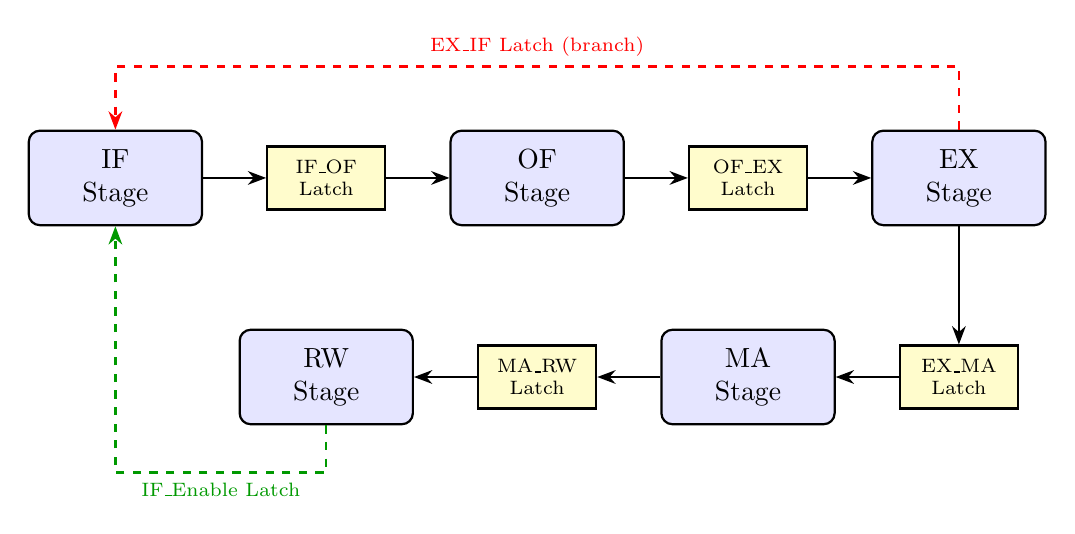
\begin{tikzpicture}[
    stage/.style={draw, rounded corners, minimum width=2.2cm, minimum height=1.2cm, align=center, fill=blue!10},
    latch/.style={draw, minimum width=1.5cm, minimum height=0.8cm, align=center, fill=yellow!20, font=\scriptsize},
    ->,>=Stealth,thick
]
    % Stages
    \node[stage] (IF) {IF\\Stage};
    \node[latch, right=0.8cm of IF] (IFOF) {IF\_OF\\Latch};
    \node[stage, right=0.8cm of IFOF] (OF) {OF\\Stage};
    \node[latch, right=0.8cm of OF] (OFEX) {OF\_EX\\Latch};
    \node[stage, right=0.8cm of OFEX] (EX) {EX\\Stage};

    % Second row
    \node[latch, below=1.5cm of EX] (EXMA) {EX\_MA\\Latch};
    \node[stage, left=0.8cm of EXMA] (MA) {MA\\Stage};
    \node[latch, left=0.8cm of MA] (MARW) {MA\_RW\\Latch};
    \node[stage, left=0.8cm of MARW] (RW) {RW\\Stage};

    % Forward arrows
    \draw (IF) -- (IFOF);
    \draw (IFOF) -- (OF);
    \draw (OF) -- (OFEX);
    \draw (OFEX) -- (EX);
    \draw (EX) -- ++(0,-0.75) -| (EXMA);
    \draw (EXMA) -- (MA);
    \draw (MA) -- (MARW);
    \draw (MARW) -- (RW);

    % EX -> IF feedback (branch)
    \draw[red, dashed, thick] (EX.north) -- ++(0,0.8) -| node[above, pos=0.25, font=\scriptsize\color{red}] {EX\_IF Latch (branch)} (IF.north);

    % RW -> IF feedback (enable)
    \draw[green!60!black, dashed, thick] (RW.south) -- ++(0,-0.6) -| node[below, pos=0.25, font=\scriptsize\color{green!60!black}] {IF\_Enable Latch} (IF.south);
\end{tikzpicture}
\caption{5-stage pipeline with inter-stage latches and feedback paths}
\end{figure}

\subsection{Latch Types Summary}

\begin{table}[H]
\centering
\begin{tabular}{@{}lll@{}}
\toprule
\textbf{Latch} & \textbf{Contents} & \textbf{Connects} \\
\midrule
\texttt{IF\_EnableLatchType} & \texttt{IF\_enable} (boolean) & RW $\rightarrow$ IF \\
\texttt{IF\_OF\_LatchType} & \texttt{instruction} (int), \texttt{OF\_enable} & IF $\rightarrow$ OF \\
\texttt{OF\_EX\_LatchType} & \texttt{instruction} (Instruction), \texttt{EX\_enable} & OF $\rightarrow$ EX \\
\texttt{EX\_MA\_LatchType} & \texttt{instruction}, \texttt{aluResult}, \texttt{MA\_enable} & EX $\rightarrow$ MA \\
\texttt{EX\_IF\_LatchType} & \texttt{isBranchEnabled}, \texttt{pc} & EX $\rightarrow$ IF \\
\texttt{MA\_RW\_LatchType} & \texttt{instruction}, \texttt{aluResult}, \texttt{Idresult}, \texttt{RW\_enable} & MA $\rightarrow$ RW \\
\bottomrule
\end{tabular}
\caption{Summary of all inter-stage latches}
\end{table}

\subsection{How Each Stage Works (Current Implementation)}

\subsubsection{Instruction Fetch (IF) --- \texttt{InstructionFetch.java}}
\begin{itemize}
    \item Checks \texttt{IF\_EnableLatch.isIF\_enable()}.
    \item If a branch was taken (from \texttt{EX\_IF\_Latch}), updates PC accordingly.
    \item Reads the instruction word from \texttt{MainMemory[PC]}.
    \item Writes the raw instruction integer to \texttt{IF\_OF\_Latch}.
    \item Increments PC by 1.
\end{itemize}

\subsubsection{Operand Fetch (OF) --- \texttt{OperandFetch.java}}
\begin{itemize}
    \item Decodes the 32-bit binary instruction (opcode, operands).
    \item Creates an \texttt{Instruction} object with \texttt{OperationType}, source and destination \texttt{Operand}s.
    \item Handles R3-Type, R2I-Type, RI-Type formats and sign extension for immediates.
    \item Writes the decoded instruction to \texttt{OF\_EX\_Latch}.
\end{itemize}

\subsubsection{Execute (EX) --- \texttt{Execute.java}}
\begin{itemize}
    \item Reads register values from the \texttt{RegisterFile}.
    \item Performs the ALU operation based on instruction type.
    \item For branches/jumps: computes target PC, sets \texttt{EX\_IF\_Latch.setBranchEnabled(true)}.
    \item Passes ALU result to \texttt{EX\_MA\_Latch}.
\end{itemize}

\subsubsection{Memory Access (MA) --- \texttt{MemoryAccess.java}}
\begin{itemize}
    \item For \texttt{load}: reads from \texttt{MainMemory[aluResult]} and stores in latch's \texttt{Idresult}.
    \item For \texttt{store}: writes register value to \texttt{MainMemory[aluResult]}.
    \item Passes instruction and results to \texttt{MA\_RW\_Latch}.
\end{itemize}

\subsubsection{Register Write (RW) --- \texttt{RegisterWrite.java}}
\begin{itemize}
    \item For arithmetic instructions: writes ALU result to destination register.
    \item For \texttt{load}: writes loaded value to destination register.
    \item For \texttt{end}: calls \texttt{Simulator.setSimulationComplete(true)}.
    \item Re-enables IF stage by setting \texttt{IF\_EnableLatch.setIF\_enable(true)}.
\end{itemize}

% ══════════════════════════════════════════════════════════════════════════════
\section{Step-by-Step Implementation Guide}
% ══════════════════════════════════════════════════════════════════════════════

\subsection{Step 1: Modify the Simulation Loop in \texttt{Simulator.java}}

This is the \textbf{most critical change}. Replace the single-cycle sequential loop with a pipelined loop.

\begin{lstlisting}[style=javastyle, caption={New pipelined simulation loop in \texttt{Simulator.java}}]
public static void simulate() {
    while (simulationComplete == false) {
        processor.getRWUnit().performRW();
        processor.getMAUnit().performMA();
        processor.getEXUnit().performEX();
        processor.getOFUnit().performOF();
        processor.getIFUnit().performIF();
        Clock.incrementClock();
    }

    // Set statistics after simulation
    Statistics.setNumberOfInstructions(instructionCount);
    Statistics.setNumberOfCycles(cycleCount);
    Statistics.setCpi(instructionCount, cycleCount);
    Statistics.setIpc(instructionCount, cycleCount);
}
\end{lstlisting}

\begin{keypoint}
\textbf{Key changes:}
\begin{enumerate}
    \item Stages are in \textbf{reverse order}: RW, MA, EX, OF, IF.
    \item Clock is incremented only \textbf{once} per iteration (not 5 times).
    \item The enable/disable mechanism in latches now controls which stages are ``active'' in each cycle.
\end{enumerate}
\end{keypoint}

\subsection{Step 2: Fix the Enable/Disable Latch Mechanism}

In the single-cycle model, the RW stage disables itself and enables IF, creating a strict chain: IF $\rightarrow$ OF $\rightarrow$ EX $\rightarrow$ MA $\rightarrow$ RW $\rightarrow$ IF $\rightarrow$ \ldots

\textbf{In the pipelined model, all stages should be active simultaneously.} This means:

\begin{itemize}
    \item \texttt{IF\_EnableLatch} should always be \texttt{true} (IF fetches every cycle unless stalled).
    \item Each latch enable bit indicates whether the \textit{downstream} stage has valid data to process.
\end{itemize}

\begin{warningbox}
Do NOT remove the enable bits. They are essential for handling:
\begin{itemize}
    \item Pipeline startup (first few cycles where later stages have no valid data).
    \item Stall cycles (when a stage is paused).
    \item Pipeline flush (when wrong-path instructions must be discarded).
\end{itemize}
\end{warningbox}

\subsubsection{Modifying \texttt{RegisterWrite.java}}
In the single-cycle model, RW re-enables IF:
\begin{lstlisting}[style=javastyle]
IF_EnableLatch.setIF_enable(true); // Remove or change this
\end{lstlisting}

In the pipelined model, IF should \textbf{always remain enabled} unless the pipeline is stalled. So in the constructor or the simulation setup, \texttt{IF\_enable} should default to \texttt{true}, and the RW stage should \textbf{not} toggle it.

\begin{lstlisting}[style=javastyle, caption={Modified RW stage (key change)}]
public void performRW() {
    if (MA_RW_Latch.isRW_enable()) {
        Instruction instruction = MA_RW_Latch.getInstruction();
        String op = instruction.getOperationType().toString();

        if (op.equals("load")) {
            containingProcessor.getRegisterFile().setValue(
                instruction.getDestinationOperand().getValue(),
                MA_RW_Latch.getIdresult());
        } else if (op.equals("end")) {
            Simulator.setSimulationComplete(true);
        } else if (!(op.equals("store") || op.equals("jmp")
                || op.equals("beq") || op.equals("blt")
                || op.equals("bne") || op.equals("bgt"))) {
            containingProcessor.getRegisterFile().setValue(
                instruction.getDestinationOperand().getValue(),
                MA_RW_Latch.getALu());
        }
        MA_RW_Latch.setRW_enable(false);
        // Do NOT set IF_EnableLatch here in pipelined mode!
    }
}
\end{lstlisting}

\subsubsection{Modifying Each Stage's Enable Logic}
Each stage should:
\begin{enumerate}
    \item Check its input latch's enable bit.
    \item If enabled, process and write to the output latch (setting the next stage's enable to \texttt{true}).
    \item If not enabled (e.g.\ bubble/NOP), set the output latch enable to \texttt{false} (propagate the bubble).
\end{enumerate}

\begin{lstlisting}[style=javastyle, caption={General pattern for each pipeline stage}]
public void performXX() {
    if (inputLatch.isXX_enable()) {
        // Process the instruction
        // Write results to output latch
        outputLatch.setNextEnable(true);
    } else {
        // Propagate bubble
        outputLatch.setNextEnable(false);
    }
}
\end{lstlisting}

\subsection{Step 3: Ensure IF Stage Is Always Active}

In the pipelined model, the IF stage should run every cycle (unless stalled). Modify the initialization:

\begin{lstlisting}[style=javastyle, caption={IF stage always enabled}]
// In Processor constructor or Simulator.setupSimulation:
IF_EnableLatch.setIF_enable(true);
// This is already the default in the constructor.

// In InstructionFetch.performIF():
// Do NOT set IF_EnableLatch.setIF_enable(false) at the end!
// The IF stage should remain enabled for the next cycle.
\end{lstlisting}

\begin{lstlisting}[style=javastyle, caption={Modified IF stage for pipelining}]
public void performIF() {
    if (IF_EnableLatch.isIF_enable()) {
        if (EX_IF_Latch.isBranchEnabled()) {
            int newPC = EX_IF_Latch.getPC();
            containingProcessor.getRegisterFile()
                .setProgramCounter(newPC);
            EX_IF_Latch.setBranchEnabled(false);
        }
        int currentPC = containingProcessor.getRegisterFile()
            .getProgramCounter();
        int newInstruction = containingProcessor.getMainMemory()
            .getWord(currentPC);
        IF_OF_Latch.setInstruction(newInstruction);
        containingProcessor.getRegisterFile()
            .setProgramCounter(currentPC + 1);
        IF_OF_Latch.setOF_enable(true);
        // DO NOT disable IF_enable!
    }
}
\end{lstlisting}

% ══════════════════════════════════════════════════════════════════════════════
\section{Implementing Data Interlocks (Hazard Detection and Stalling)}
% ══════════════════════════════════════════════════════════════════════════════

\subsection{What is a Data Hazard?}

A \textbf{data hazard} occurs when an instruction in the OF stage needs to read a register that a preceding instruction (currently in EX, MA, or RW) has not yet written back to. This is a \textbf{Read-After-Write (RAW)} hazard.

\textbf{Example:}
\begin{lstlisting}[style=asmstyle]
addi %x0, 5, %x3     ; writes to x3
add  %x3, %x4, %x5   ; reads x3 -- DATA HAZARD!
\end{lstlisting}

When the \texttt{add} instruction is in the OF stage trying to read \texttt{x3}, the \texttt{addi} instruction may still be in EX, MA, or RW and has \textit{not yet} written the new value of \texttt{x3} to the register file.

\subsection{Where to Detect Hazards}

Detect hazards in the \textbf{OF stage} (\texttt{OperandFetch.java}). The OF stage decodes the instruction and knows which registers it needs. It must check if any instruction in EX, MA, or RW stages will write to those registers.

\subsection{How to Track Destination Registers of In-Flight Instructions}

You need to know what registers are being written by instructions currently in the pipeline. Two common approaches:

\subsubsection{Approach A: Check the Latches Directly}

Inspect the \texttt{OF\_EX\_Latch}, \texttt{EX\_MA\_Latch}, and \texttt{MA\_RW\_Latch} to read the instructions in later stages and check their destination registers.

\subsubsection{Approach B: Maintain a ``Busy'' Bit Array (Scoreboard)}

Maintain an array \texttt{boolean[] registerBusy = new boolean[32]} in the \texttt{RegisterFile}:
\begin{itemize}
    \item When OF dispatches an instruction that writes to register \texttt{rd}, set \texttt{registerBusy[rd] = true}.
    \item When RW writes back to register \texttt{rd}, set \texttt{registerBusy[rd] = false}.
    \item In OF, before reading source registers, check if \texttt{registerBusy[rs1]} or \texttt{registerBusy[rs2]} is true. If so, \textbf{stall}.
\end{itemize}

\begin{keypoint}
Approach B (scoreboard) is simpler and is \textbf{recommended} for this assignment.
\end{keypoint}

\subsection{Implementing the Stall}

When a data hazard is detected in OF:

\begin{enumerate}
    \item \textbf{OF does NOT write to OF\_EX latch} --- it keeps its input unchanged.
    \item \textbf{OF\_EX\_Latch enable is set to false} --- inject a ``bubble'' (NOP) into EX.
    \item \textbf{IF is stalled} --- the IF stage must not fetch a new instruction. Set \texttt{IF\_EnableLatch.setIF\_enable(false)}.
    \item \textbf{Decrement PC} back by 1, or simply do not let IF advance. The simplest approach: just disable IF by not enabling it.
\end{enumerate}

\begin{lstlisting}[style=javastyle, caption={Hazard detection and stalling in OF stage}]
public void performOF() {
    if (IF_OF_Latch.isOF_enable()) {
        // Decode the instruction as before...
        Instruction inst = decode(IF_OF_Latch.getInstruction());

        // Identify source registers
        int src1Reg = -1, src2Reg = -1;
        if (inst.getSourceOperand1() != null
            && inst.getSourceOperand1().getOperandType()
               == OperandType.Register) {
            src1Reg = inst.getSourceOperand1().getValue();
        }
        if (inst.getSourceOperand2() != null
            && inst.getSourceOperand2().getOperandType()
               == OperandType.Register) {
            src2Reg = inst.getSourceOperand2().getValue();
        }

        // Check for hazards (busy registers)
        RegisterFile rf = containingProcessor.getRegisterFile();
        boolean hazard = false;
        if (src1Reg >= 0 && rf.isRegisterBusy(src1Reg))
            hazard = true;
        if (src2Reg >= 0 && rf.isRegisterBusy(src2Reg))
            hazard = true;

        if (hazard) {
            // STALL: inject bubble into EX
            OF_EX_Latch.setEX_enable(false);
            // Keep IF stalled (do not fetch next instruction)
            IF_EnableLatch.setIF_enable(false);
            // Increment data hazard stall counter
            Statistics.incrementDataHazardStalls();
        } else {
            // No hazard: proceed normally
            OF_EX_Latch.setInstruction(inst);
            OF_EX_Latch.setEX_enable(true);
            IF_OF_Latch.setOF_enable(false);

            // Mark destination register as busy
            int destReg = getDestRegister(inst);
            if (destReg > 0) { // don't mark x0
                rf.setRegisterBusy(destReg, true);
            }
        }
    } else {
        // No valid instruction: propagate bubble
        OF_EX_Latch.setEX_enable(false);
    }
}
\end{lstlisting}

\begin{warningbox}
\textbf{Special cases for hazard detection:}
\begin{itemize}
    \item \texttt{store} instructions: the ``destination'' operand in the Instruction object is actually the register whose contents provide the memory address. The actual register to check for reads is \texttt{sourceOperand1} (rs1). Be careful about which registers count as ``sources.''
    \item \texttt{jmp} instructions: may read from a register in the destination operand field. Handle accordingly.
    \item Branches (\texttt{beq}, \texttt{bne}, \texttt{blt}, \texttt{bgt}): both \texttt{sourceOperand1} and \texttt{sourceOperand2} are registers to compare.
    \item \texttt{x0} is hardwired to 0 and should never be marked as busy.
    \item \texttt{x31} may be written implicitly (by \texttt{div}, \texttt{mul}, shift instructions). Consider whether to mark it busy.
\end{itemize}
\end{warningbox}

\subsection{Adding Busy Bits to \texttt{RegisterFile.java}}

\begin{lstlisting}[style=javastyle, caption={Additions to \texttt{RegisterFile.java}}]
public class RegisterFile {
    int[] registerFile;
    int programCounter;
    boolean[] busy; // NEW

    public RegisterFile() {
        registerFile = new int[32];
        busy = new boolean[32]; // all false initially
    }

    public boolean isRegisterBusy(int regNum) {
        return busy[regNum];
    }

    public void setRegisterBusy(int regNum, boolean val) {
        if (regNum != 0) // x0 is always 0, never busy
            busy[regNum] = val;
    }
    // ... existing methods unchanged ...
}
\end{lstlisting}

\subsection{Clearing Busy Bits in RW Stage}

In \texttt{RegisterWrite.java}, after writing the result to the register, clear the busy bit:

\begin{lstlisting}[style=javastyle, caption={Clearing busy bits in RW stage}]
// After writing to register rd:
containingProcessor.getRegisterFile()
    .setRegisterBusy(rd, false);
\end{lstlisting}

% ══════════════════════════════════════════════════════════════════════════════
\section{Implementing Control Interlocks (Branch Handling)}
% ══════════════════════════════════════════════════════════════════════════════

\subsection{What is a Control Hazard?}

A \textbf{control hazard} occurs when a branch or jump instruction is in the pipeline, and the processor has already fetched subsequent instructions that may be on the \textbf{wrong execution path}.

In this simulator, branches are resolved in the \textbf{EX stage}. By the time EX determines that a branch is taken, the IF and OF stages have already fetched and decoded 1--2 instructions from the \textbf{fall-through path} (the path assuming the branch is not taken).

\subsection{Pipeline Timing of a Branch}

\begin{table}[H]
\centering
\begin{tabular}{@{}lcccccc@{}}
\toprule
\textbf{Cycle} & \textbf{1} & \textbf{2} & \textbf{3} & \textbf{4} & \textbf{5} & \textbf{6} \\
\midrule
Branch instr. & IF & OF & EX & MA & RW & \\
Instr. at PC+1 & & IF & OF & \textit{flush} & & \\
Instr. at PC+2 & & & IF & \textit{flush} & & \\
Target instr. & & & & IF & OF & EX \\
\bottomrule
\end{tabular}
\caption{Branch instruction timing in a 5-stage pipeline}
\end{table}

When the branch is resolved as \textbf{taken} in cycle 3 (EX stage), the two instructions already fetched (at PC+1 and PC+2) must be \textbf{flushed} (invalidated).

\subsection{Implementing the Flush}

When EX detects a taken branch:

\begin{enumerate}
    \item Set \texttt{EX\_IF\_Latch.setBranchEnabled(true)} and \texttt{EX\_IF\_Latch.setPC(targetPC)}.
    \item \textbf{Invalidate the IF\_OF latch} (the instruction in OF is on the wrong path): set \texttt{IF\_OF\_Latch.setOF\_enable(false)}.
    \item \textbf{Invalidate the OF\_EX latch} (the instruction about to enter EX is also wrong): set \texttt{OF\_EX\_Latch.setEX\_enable(false)}.
\end{enumerate}

\begin{lstlisting}[style=javastyle, caption={Branch handling in EX stage}]
// When a branch is taken (e.g., beq condition is true):
alu = pcnow + immed;
EX_IF_Latch.setBranchEnabled(true);
EX_IF_Latch.setPC(alu);

// Flush pipeline: invalidate instructions in IF and OF
IF_OF_Latch.setOF_enable(false);
// The OF_EX_Latch will be set to false by default
// since OF won't produce valid output

// Increment wrong-path counter
Statistics.incrementWrongBranchCount();
\end{lstlisting}

\begin{keypoint}
For \textbf{unconditional jumps} (\texttt{jmp}), the branch is \textbf{always taken}, so you always flush. For conditional branches, you only flush when the condition evaluates to true.
\end{keypoint}

\begin{tipbox}
The number of wrong-path instructions that entered the pipeline corresponds to how many instructions were fetched and started processing before the branch was resolved. In a simple 5-stage pipeline with branch resolution at EX, this is typically \textbf{2 instructions} per taken branch (the ones in IF and OF stages).
\end{tipbox}

\subsection{Counting Wrong-Path Instructions}

Each time a branch is taken and the pipeline is flushed, count how many instructions on the wrong path entered the pipeline. This is the number of valid instructions in stages between IF and EX at the time of the branch resolution:

\begin{lstlisting}[style=javastyle, caption={Counting wrong branch entries}]
// In Execute.java, when branch is taken:
int wrongPathCount = 0;
if (IF_OF_Latch.isOF_enable()) wrongPathCount++;
// The instruction that was in IF during this cycle
// (it will have been fetched before we noted the branch)
wrongPathCount++; // IF always fetches if enabled

Statistics.addWrongBranchInstructions(wrongPathCount);
\end{lstlisting}

% ══════════════════════════════════════════════════════════════════════════════
\section{Modifications to \texttt{Statistics.java}}
% ══════════════════════════════════════════════════════════════════════════════

Add new counters for the required statistics:

\begin{lstlisting}[style=javastyle, caption={Updated \texttt{Statistics.java}}]
public class Statistics {
    static int numberOfInstructions;
    static int numberOfCycles;
    static float ipc;
    static float cpi;
    static int dataHazardStalls;     // NEW
    static int wrongBranchCount;     // NEW

    // Increment methods
    public static void incrementDataHazardStalls() {
        dataHazardStalls++;
    }

    public static void incrementWrongBranchCount() {
        wrongBranchCount++;
    }

    // Getters
    public static int getDataHazardStalls() {
        return dataHazardStalls;
    }

    public static int getWrongBranchCount() {
        return wrongBranchCount;
    }

    public static void printStatistics(String statFile) {
        try {
            PrintWriter writer = new PrintWriter(statFile);
            writer.println("Number of instructions = "
                + numberOfInstructions);
            writer.println("Number of cycles = "
                + numberOfCycles);
            writer.println("CPI = " + cpi);
            writer.println("IPC = " + ipc);
            writer.println("Data hazard stalls = "
                + dataHazardStalls);
            writer.println("Wrong branch instructions = "
                + wrongBranchCount);
            writer.close();
        } catch (Exception e) {
            Misc.printErrorAndExit(e.getMessage());
        }
    }
    // ... existing setters remain ...
}
\end{lstlisting}

% ══════════════════════════════════════════════════════════════════════════════
\section{Handling the \texttt{end} Instruction in a Pipeline}
% ══════════════════════════════════════════════════════════════════════════════

\begin{warningbox}
In the pipelined model, when an \texttt{end} instruction is fetched, the simulator must \textbf{not stop immediately}. The \texttt{end} instruction must flow through all 5 stages (IF $\rightarrow$ OF $\rightarrow$ EX $\rightarrow$ MA $\rightarrow$ RW) before \texttt{setSimulationComplete(true)} is called. Meanwhile, the IF stage may continue fetching instructions after \texttt{end}, but those are irrelevant as long as the simulation terminates correctly when \texttt{end} reaches RW.
\end{warningbox}

One approach: when the OF stage decodes an \texttt{end} instruction, disable IF to prevent further fetches:

\begin{lstlisting}[style=javastyle]
case end:
    // In OF stage: stop fetching
    IF_EnableLatch.setIF_enable(false);
    break;
\end{lstlisting}

The \texttt{end} instruction then propagates through EX, MA, and RW. When RW processes it, it calls \texttt{Simulator.setSimulationComplete(true)}.

% ══════════════════════════════════════════════════════════════════════════════
\section{Complete Modified File Summary}
% ══════════════════════════════════════════════════════════════════════════════

\begin{table}[H]
\centering
\begin{tabular}{@{}lp{10cm}@{}}
\toprule
\textbf{File} & \textbf{Changes Required} \\
\midrule
\texttt{Simulator.java} & Rewrite \texttt{simulate()} to call stages in reverse order with a single \texttt{Clock.incrementClock()} per iteration. \\
\texttt{InstructionFetch.java} & Do not disable \texttt{IF\_enable} at end of \texttt{performIF()}. Handle stall signal (when OF requests a stall, IF must not advance PC). \\
\texttt{OperandFetch.java} & Add hazard detection logic. Check busy registers. If hazard: stall (inject bubble, disable IF). Add counter increment for data hazard stalls. \\
\texttt{Execute.java} & On taken branch: flush IF\_OF and OF\_EX latches. Increment wrong-path counter. Fix pcnow calculation for pipelined operation. \\
\texttt{MemoryAccess.java} & Propagate bubbles (if MA\_enable is false, set RW\_enable false). \\
\texttt{RegisterWrite.java} & Remove \texttt{IF\_EnableLatch.setIF\_enable(true)}. Clear busy bits after writeback. \\
\texttt{RegisterFile.java} & Add \texttt{boolean[] busy} array with \texttt{isRegisterBusy()} and \texttt{setRegisterBusy()} methods. \\
\texttt{Statistics.java} & Add \texttt{dataHazardStalls} and \texttt{wrongBranchCount} counters with increment methods and print support. \\
\texttt{IF\_OF\_LatchType.java} & Possibly add a field to store the PC of the fetched instruction (useful for branch target calculation). \\
\texttt{OF\_EX\_LatchType.java} & Possibly add a field to store the PC (for EX stage branch target computation). \\
\bottomrule
\end{tabular}
\caption{Summary of all files to modify}
\end{table}

% ══════════════════════════════════════════════════════════════════════════════
\section{Handling the PC Correctly in a Pipeline}
% ══════════════════════════════════════════════════════════════════════════════

In the single-cycle model, the EX stage computes \texttt{pcnow} as:
\begin{lstlisting}[style=javastyle]
int pcnow = containingProcessor.getRegisterFile()
    .programCounter - 1;
\end{lstlisting}

This works because in the single-cycle model, PC was just incremented by IF and no other instruction has touched it.

\begin{warningbox}
In the pipelined model, \textbf{PC keeps advancing every cycle} as IF fetches new instructions. By the time an instruction reaches EX, the PC has already moved ahead by 2 or more. The method above will give the \textbf{wrong} value.
\end{warningbox}

\textbf{Solution:} Store the PC of each instruction \textbf{in the latches} as it flows through the pipeline.

\begin{enumerate}
    \item In \texttt{IF\_OF\_LatchType}, add a field \texttt{int instructionPC} and set it during IF.
    \item Carry this PC through each latch: OF\_EX, EX\_MA, MA\_RW.
    \item In the Instruction object itself, use the existing \texttt{programCounter} field --- set it during OF.
\end{enumerate}

\begin{lstlisting}[style=javastyle, caption={Storing PC in the instruction during OF}]
// In OperandFetch.performOF():
inst.setProgramCounter(IF_OF_Latch.getInstructionPC());
\end{lstlisting}

\begin{lstlisting}[style=javastyle, caption={Using stored PC in EX for branch target}]
// In Execute.performEX():
int pcnow = inst.getProgramCounter();
// Branch target: alu = pcnow + immed;
\end{lstlisting}

% ══════════════════════════════════════════════════════════════════════════════
\section{Testing and Verification}
% ══════════════════════════════════════════════════════════════════════════════

\subsection{Test Cases}

The provided test cases (from Assignment 3) must still produce correct results:

\begin{table}[H]
\centering
\begin{tabular}{@{}lp{8cm}@{}}
\toprule
\textbf{Benchmark} & \textbf{Description} \\
\midrule
\texttt{fibonacci.asm} & Computes first 10 Fibonacci numbers, stores them on the stack. Loop-heavy with moderate data dependencies. \\
\texttt{descending.asm} & Bubble sort of 8 elements in descending order. Nested loops with many branches and data dependencies on loaded values. \\
\texttt{prime.asm} & Checks if 11 is prime by trial division. Uses \texttt{div} and checks \texttt{x31} (remainder). \\
\texttt{evenorodd.asm} & Checks if 11 is even or odd. Very short, uses \texttt{divi} and \texttt{beq}. \\
\texttt{palindrome.asm} & Checks if 4567654 is a palindrome. Loop with \texttt{divi}/\texttt{muli} and \texttt{x31}. \\
\bottomrule
\end{tabular}
\caption{Benchmark programs and their characteristics}
\end{table}

\subsection{How to Build and Run}

\begin{lstlisting}[style=asmstyle, caption={Building and running the simulator}]
# Build
cd supporting_files
ant build

# Create JAR
ant make-jar

# Run on a test case
java -jar jars/simulator.jar \
    src/configuration/config.xml \
    output_stats.txt \
    test_cases/fibonacci.out

# Check hash value against expected
cat test_cases/fibonacci.expected
\end{lstlisting}

\subsection{Using the Test Script}

\begin{lstlisting}[style=asmstyle]
python test_zip.py <path-to-your-zip>
\end{lstlisting}

\subsection{Verification Checklist}

\begin{enumerate}[label=$\square$]
    \item All 5 test cases produce the \textbf{correct hash value} (same as Assignment 3).
    \item The \textbf{final register and memory states} are identical to the single-cycle model.
    \item The cycle count is $\geq$ the instruction count (pipeline overhead from hazards).
    \item Data hazard stall count is reasonable:
    \begin{itemize}
        \item \texttt{evenorodd}: few stalls (very short program).
        \item \texttt{descending}: many stalls (loads followed by comparisons).
    \end{itemize}
    \item Wrong-branch-path count correlates with number of taken branches.
\end{enumerate}

% ══════════════════════════════════════════════════════════════════════════════
\section{Writing the Report}
% ══════════════════════════════════════════════════════════════════════════════

\subsection{Required Table}

\begin{table}[H]
\centering
\begin{tabular}{@{}lccc@{}}
\toprule
\textbf{Benchmark} & \textbf{Cycles} & \textbf{OF Stalls (Data)} & \textbf{Wrong Branch Entries} \\
\midrule
\texttt{fibonacci} & --- & --- & --- \\
\texttt{descending} & --- & --- & --- \\
\texttt{prime} & --- & --- & --- \\
\texttt{evenorodd} & --- & --- & --- \\
\texttt{palindrome} & --- & --- & --- \\
\bottomrule
\end{tabular}
\caption{Template for the required benchmark results table (fill in after running)}
\end{table}

\subsection{Observations to Comment On}

\begin{itemize}
    \item \textbf{Data Hazard Stalls:} Programs with many back-to-back dependent arithmetic instructions (like Fibonacci with \texttt{add} followed immediately by using the result) will have more stalls. Load-use hazards (e.g., \texttt{load} followed by an instruction using the loaded value) are particularly common.
    \item \textbf{Wrong Branch Entries:} Programs with loops (Fibonacci, descending sort) will have more taken branches since the loop-back branch is taken on every iteration except the last. The descending sort, with its nested loops, will have the most.
    \item \textbf{CPI Analysis:} Ideal CPI for a pipeline is 1.0. The actual CPI will be higher due to stall cycles and flush cycles. You can break down: $\text{CPI} = 1 + \frac{\text{stall cycles} + \text{flush cycles}}{\text{total instructions}}$.
\end{itemize}

% ══════════════════════════════════════════════════════════════════════════════
\section{Common Pitfalls and Debugging Tips}
% ══════════════════════════════════════════════════════════════════════════════

\begin{enumerate}
    \item \textbf{Latch Overwrite Problem:} If you process IF before RW, the data written by IF into the IF\_OF latch gets consumed by OF in the same cycle. Always process in reverse order.

    \item \textbf{Off-by-One in PC:} In the pipelined model, the PC stored with an instruction should be the PC \textit{at the time of fetch}, not the current global PC. Store PC in the latch.

    \item \textbf{Forgetting to Propagate Bubbles:} If EX has no valid instruction (EX\_enable is false), it must set MA\_enable to false. Otherwise, the MA stage may process stale data from a previous cycle.

    \item \textbf{Register x0 Marked Busy:} Never mark x0 as busy. It is hardwired to 0.

    \item \textbf{Branch + Data Hazard Interaction:} If a branch instruction has a data hazard (its source register is being written by a preceding instruction), the branch must stall. Don't flush on a stalled branch.

    \item \textbf{Counting Instructions vs. Cycles:} In the pipelined model, instruction count and cycle count are different. Be careful to count only \textit{committed} (completed through RW) instructions, not fetched instructions.

    \item \textbf{Store Instruction Operand Confusion:} In the ISA, \texttt{store} has \texttt{rd} as the base address register and \texttt{rs1} as the data source. The decoded instruction swaps these in the Operand fields. Be careful when checking for hazards.

    \item \textbf{End Instruction in Pipeline:} If \texttt{end} is fetched but more instructions come after it, those must be discarded or their effects made irrelevant by stopping at RW of \texttt{end}.
\end{enumerate}

% ══════════════════════════════════════════════════════════════════════════════
\section{Summary of Changes at a Glance}
% ══════════════════════════════════════════════════════════════════════════════

\begin{tcolorbox}[colback=blue!5!white, colframe=blue!50!black, title=\textbf{Complete Change Checklist}]
\begin{enumerate}
    \item[\textbf{1.}] \textbf{Simulator.java}: Reverse stage order, single clock increment per cycle.
    \item[\textbf{2.}] \textbf{RegisterFile.java}: Add \texttt{busy[]} array, getter/setter.
    \item[\textbf{3.}] \textbf{IF\_OF\_LatchType.java}: Add \texttt{instructionPC} field.
    \item[\textbf{4.}] \textbf{InstructionFetch.java}: Store PC in latch, keep IF always enabled.
    \item[\textbf{5.}] \textbf{OperandFetch.java}: Add hazard detection, stall logic, busy-bit setting.
    \item[\textbf{6.}] \textbf{Execute.java}: Fix PC calculation (use stored PC), add pipeline flush on taken branch.
    \item[\textbf{7.}] \textbf{MemoryAccess.java}: Propagate bubbles when MA\_enable is false.
    \item[\textbf{8.}] \textbf{RegisterWrite.java}: Remove IF re-enable, clear busy bits on writeback.
    \item[\textbf{9.}] \textbf{Statistics.java}: Add \texttt{dataHazardStalls}, \texttt{wrongBranchCount} counters.
    \item[\textbf{10.}] \textbf{All stages}: Handle enable=false case (propagate bubble to next latch).
\end{enumerate}
\end{tcolorbox}

\newpage
\appendix

% ══════════════════════════════════════════════════════════════════════════════
\section{ToyRISC ISA Quick Reference}
% ══════════════════════════════════════════════════════════════════════════════

\subsection{Instruction Formats}

\begin{table}[H]
\centering
\begin{tabular}{@{}llllll@{}}
\toprule
\textbf{Format} & \textbf{Bits [31:27]} & \textbf{Bits [26:22]} & \textbf{Bits [21:17]} & \textbf{Bits [16:5]} & \textbf{Bits [4:0]} \\
\midrule
R3-Type  & opcode (5) & rs1 (5) & rs2 (5) & unused (12) & rd (5) \\
R2I-Type & opcode (5) & rs1 (5) & rd (5) & \multicolumn{2}{l}{immediate (17)} \\
RI-Type  & opcode (5) & rd (5) & \multicolumn{3}{l}{immediate (22)} \\
\bottomrule
\end{tabular}
\caption{ToyRISC instruction format encodings}
\end{table}

\subsection{Complete Opcode Table}

\begin{longtable}{@{}lllp{6cm}@{}}
\toprule
\textbf{Operation} & \textbf{Opcode} & \textbf{Format} & \textbf{Description} \\
\midrule
\endfirsthead
\toprule
\textbf{Operation} & \textbf{Opcode} & \textbf{Format} & \textbf{Description} \\
\midrule
\endhead
\texttt{add}  & 00000 & R3   & rd = rs1 + rs2 \\
\texttt{addi} & 00001 & R2I  & rd = rs1 + imm \\
\texttt{sub}  & 00010 & R3   & rd = rs1 - rs2 \\
\texttt{subi} & 00011 & R2I  & rd = rs1 - imm \\
\texttt{mul}  & 00100 & R3   & rd = rs1 $\times$ rs2 \\
\texttt{muli} & 00101 & R2I  & rd = rs1 $\times$ imm \\
\texttt{div}  & 00110 & R3   & rd = rs1 / rs2; x31 = rs1 \% rs2 \\
\texttt{divi} & 00111 & R2I  & rd = rs1 / imm; x31 = rs1 \% imm \\
\texttt{and}  & 01000 & R3   & rd = rs1 \& rs2 \\
\texttt{andi} & 01001 & R2I  & rd = rs1 \& imm \\
\texttt{or}   & 01010 & R3   & rd = rs1 $|$ rs2 \\
\texttt{ori}  & 01011 & R2I  & rd = rs1 $|$ imm \\
\texttt{xor}  & 01100 & R3   & rd = rs1 $\oplus$ rs2 \\
\texttt{xori} & 01101 & R2I  & rd = rs1 $\oplus$ imm \\
\texttt{slt}  & 01110 & R3   & rd = (rs1 $<$ rs2) ? 1 : 0 \\
\texttt{slti} & 01111 & R2I  & rd = (rs1 $<$ imm) ? 1 : 0 \\
\texttt{sll}  & 10000 & R3   & rd = rs1 $\ll$ rs2 \\
\texttt{slli} & 10001 & R2I  & rd = rs1 $\ll$ imm \\
\texttt{srl}  & 10010 & R3   & rd = rs1 $\ggg$ rs2 (logical) \\
\texttt{srli} & 10011 & R2I  & rd = rs1 $\ggg$ imm (logical) \\
\texttt{sra}  & 10100 & R3   & rd = rs1 $\gg$ rs2 (arithmetic) \\
\texttt{srai} & 10101 & R2I  & rd = rs1 $\gg$ imm (arithmetic) \\
\texttt{load} & 10110 & R2I  & rd = Mem[rs1 + imm] \\
\texttt{store}& 10111 & R2I  & Mem[rd + imm] = rs1 \\
\texttt{jmp}  & 11000 & RI   & PC = PC + rd + imm \\
\texttt{beq}  & 11001 & R2I  & if rs1 = rd: PC = PC + imm \\
\texttt{bne}  & 11010 & R2I  & if rs1 $\neq$ rd: PC = PC + imm \\
\texttt{blt}  & 11011 & R2I  & if rs1 $<$ rd: PC = PC + imm \\
\texttt{bgt}  & 11100 & R2I  & if rs1 $>$ rd: PC = PC + imm \\
\texttt{end}  & 11101 & RI   & Terminate execution \\
\bottomrule
\end{longtable}

\subsection{Registers}

\begin{table}[H]
\centering
\begin{tabular}{@{}lll@{}}
\toprule
\textbf{Register} & \textbf{Encoding} & \textbf{Purpose} \\
\midrule
x0 & 00000 & Hardwired zero \\
x1 & 00001 & Stack pointer \\
x2 & 00010 & Frame pointer \\
x3--x30 & 00011--11110 & General purpose \\
x31 & 11111 & Special (overflow, remainder, shifted-out bits) \\
PC & --- & Program counter \\
\bottomrule
\end{tabular}
\caption{ToyRISC register file}
\end{table}

% ══════════════════════════════════════════════════════════════════════════════
\section{Sample Benchmark: Fibonacci Walkthrough}
% ══════════════════════════════════════════════════════════════════════════════

The Fibonacci benchmark illustrates common hazards:

\begin{lstlisting}[style=asmstyle, caption={fibonacci.asm (excerpt)}]
loop:
    add  %x3, %x4, %x5    ; x5 = x3 + x4
    store %x5, 0, %x7     ; store x5 -> uses x5 (DATA HAZARD!)
    subi %x7, 1, %x7      ; x7 = x7 - 1
    addi %x8, 1, %x8      ; x8 = x8 + 1
    add  %x0, %x4, %x3    ; x3 = x4
    add  %x0, %x5, %x4    ; x4 = x5 (DATA HAZARD on x5!)
    jmp  for               ; CONTROL HAZARD
\end{lstlisting}

\textbf{Data hazards:}
\begin{itemize}
    \item \texttt{store \%x5} depends on \texttt{add \ldots, \%x5} (1 instruction apart).
    \item \texttt{add \ldots, \%x4} at line 6 depends on \texttt{add \ldots, \%x3} which writes x3 (though x4 is the source here, it was written 5 instructions prior, so no hazard).
\end{itemize}

\textbf{Control hazard:}
\begin{itemize}
    \item \texttt{jmp for} causes a flush every iteration (unconditional jump is always taken).
\end{itemize}

\end{document}
